\begin{figure}[!h]
  %\centering
  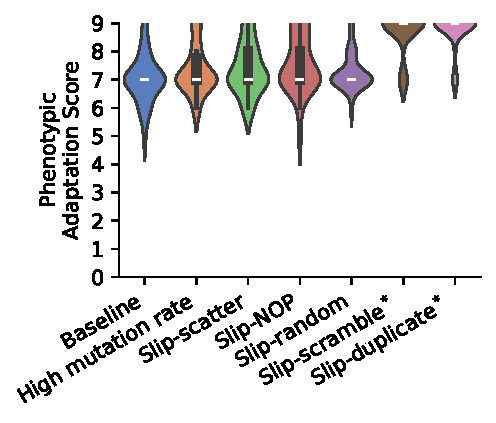
\includegraphics[height=3in,trim={0.2cm 0 0.2cm 0},clip]{binder/binder/teeplots/env=static+hue=treatment+inner=box+kind=violin+palette=muted+viz=catplot+x=treatment+y=tasks-present+ext=.pdf}%
   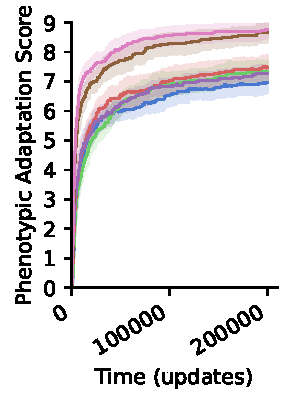
\includegraphics[height=3in,trim={0.96cm -0.64cm 0 0},clip]{binder/binder/teeplots/env=static+errorbar=ci+hue=treatment+kind=line+palette=muted+viz=relplot+x=time+y=tasks-present+ext=.pdf}

   \vspace{-2ex}

  \caption{\textbf{Slip-scramble and slip-duplicate treatments facilitate adaptive evolution.}
  \small Violin plot (left) shows distribution of the phenotypic adaptation scores for final dominant genotypes.
  Time series (right) shows progression of phenotypic adaptation score along lineages of final dominant genotypes;
  color-coding corresponds to violin plots.
  Asterisk (*) markers indicate treatments with significantly higher phenotypic adaptation scores compared to baseline.
  Simulation time unit is ``updates,'' corresponding to evaluation of approximately 30 genome sites per organism.
  Data shown from second-phase experiments.
}
  \label{fig:results_panels}
\end{figure}
